%*******************************************************************************
%*********************************** Second Chapter ****************************
%*******************************************************************************

%Title of the Second Chapter
\chapter{Quantum Optics of Quantum Gases}  

\ifpdf
    \graphicspath{{Chapter2/Figs/Raster/}{Chapter2/Figs/PDF/}{Chapter2/Figs/}}
\else
    \graphicspath{{Chapter2/Figs/Vector/}{Chapter2/Figs/}}
\fi


%********************************** % First Section  ****************************

\section{Ultracold Atoms in Optical Lattices}

%********************************** % Second Section  ***************************

\section{Quantum Optics of Quantum Gases}

Having introduced and described the behaviour of ultracold bosons
trapped and manipulated using classical light, it is time to extend
the discussion to quantized optical fields. We will first derive a
general Hamiltonian that describes the coupling of atoms with
far-detuned optical beams \cite{mekhov2012}. This will serve as the
basis from which we explore the system in different parameter regimes,
such as nondestructive measurement in free space or quantum
measurement backaction in a cavity.

We consider $N$ two-level atoms in an optical lattice with $M$
sites. For simplicity we will restrict our attention to spinless
bosons, although it is straightforward to generalise to fermions,
which yields its own set of interesting quantum phenomena
\cite{atoms2015, mazzucchi2016, mazzucchi2016af}, and other spin
particles. The theory can be also be generalised to continuous
systems, but the restriction to optical lattices is convenient for a
variety of reasons. Firstly, it allows us to precisely describe a
many-body atomic state over a broad range of parameter values due to
the inherent tunability of such lattices. Furthermore, this model is
capable of describing a range of different experimental setups ranging
from a small number of sites with a large filling factor (e.g.~BECs
trapped in a double-well potential) to a an extended multi-site
lattice with a low filling factor (e.g.~a system with one atom per
site will exhibit the Mott insulator to superfluid quantum phase
transition). \mynote{extra fermion citations, Piazza? Look up Gabi's
  AF paper.}

\mynote{Potentially some more crap, but come to think of it the
  content will strongly depend on what was included in the preceding
  section on plain ultracold bosons}

As we have seen in the previous section, an optical lattice can be
formed with classical light beams that form standing waves. Depending
on the detuning with respect to the atomic resonance, the nodes or
antinodes form the lattice sites in which atoms accumulate. As shown
in Fig. \ref{fig:LatticeDiagram} the trapped bosons (green) are
illuminated with a coherent probe beam (red) and scatter light into a
different mode (blue) which is then measured with a detector. The most
straightforward measurement is to simply count the number of photons
with a photodetector, but it is also possible to perform a quadrature
measurement by using a homodyne detection scheme. The experiment can
be performed in free space where light can scatter in any
direction. The atoms can also be placed inside a cavity which has the
advantage of being able to enhance light scattering in a particular
direction. Furthermore, cavities allow for the formation of a fully
quantum potential in contrast to the classical lattice trap.

\begin{figure}[htbp!]
  \centering
  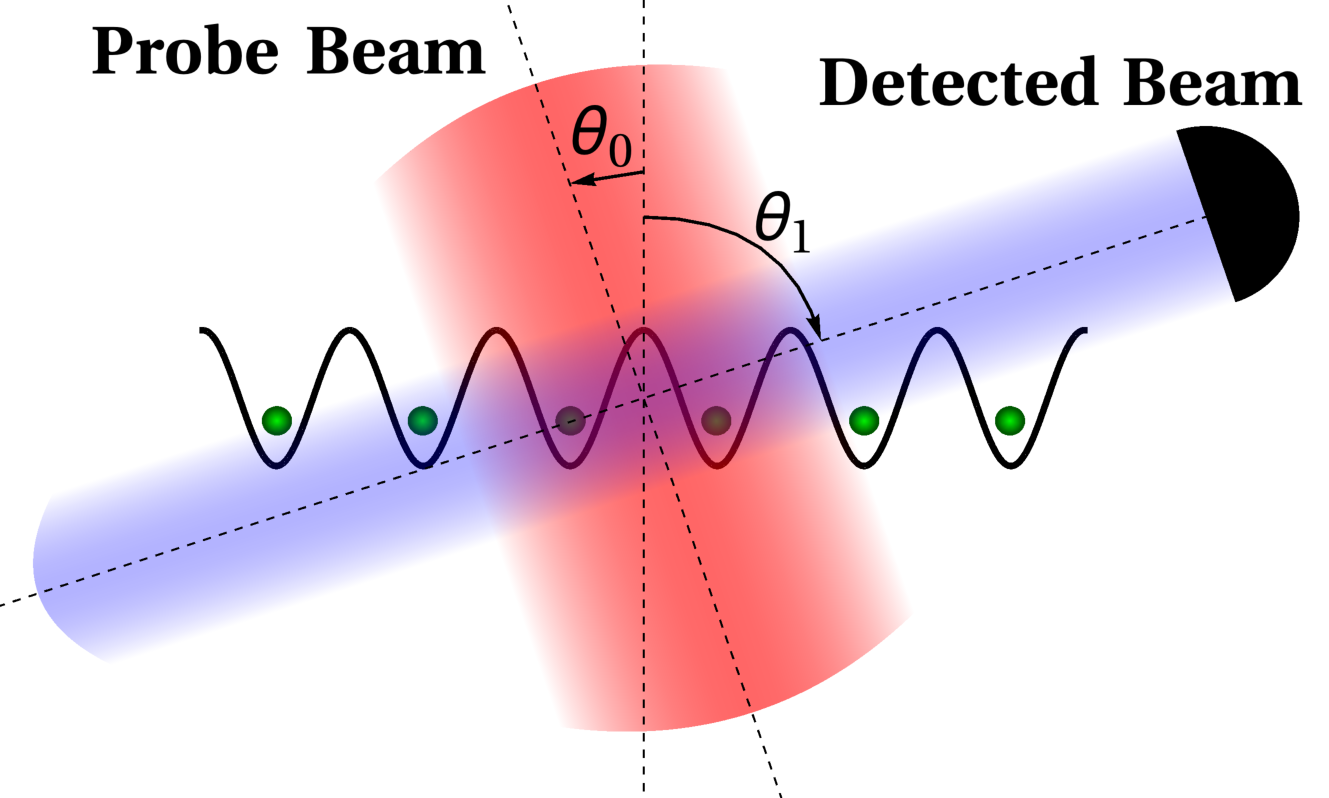
\includegraphics[width=1.0\textwidth]{LatticeDiagram}
  \caption[Experimental Setup]{Atoms (green) trapped in an optical
    lattice are illuminated by a coherent probe beam (red). The light
    scatters (blue) in free space or into a cavity and is measured by
    a detector. If the experiment is in free space light can scatter
    in any direction. A cavity on the other hand enhances scattering
    in one particular direction.}
  \label{fig:LatticeDiagram}
\end{figure}

For simplicity, we will be considering one-dimensional lattices most
of the time. However, the model itself is derived for any number of
dimensions and since none of our arguments will ever rely on
dimensionality our results straightforwardly generalise to 2- and 3-D
systems. This simplification allows us to present a much simpler
picture of the physical setup where we only need to concern ourselves
with a single angle for each optical mode. As shown in
Fig. \ref{fig:LatticeDiagram} the angle between the normal to the
lattice and the probe and detected beam are denoted by $\theta_0$ and
$\theta_1$ respectively. We will consider these angles to be tunable
although the same effect can be achieved by varying the wavelength of
the light modes. However, it is much more intuitive to consider
variable angles in our model as this lends itself to a simpler
geometrical representation.

\subsection{Derivation of the Hamiltonian}

A general many-body Hamiltonian coupled to a quantized light field in
second quantized can be separated into three parts,
\begin{equation}
\label{eq:FullH}
  \H = \H_f + \H_a + \H_{fa}.
\end{equation}
The term $\H_f$ represents the optical part of the Hamiltonian,
\begin{equation}
\label{eq:Hf}
  \H_f = \sum_l \hbar \omega_l \ad_l \a_l -
  i \hbar \sum_l \left( \eta_l^* \a_l - \eta_l \ad \right).
\end{equation}
The operators $\a_l$ ($\ad$) are the annihilation (creation) operators
of light modes with frequencies $\omega_l$, wave vectors $\b{k}_l$,
and mode functions $u_l(\b{r})$, which can be pumped by coherent
fields with amplitudes $\eta_l$. The second part of the Hamiltonian,
$\H_a$, is the matter-field component given by
\begin{equation}
\label{eq:Ha}
  \H_a = \int \mathrm{d}^3 \b{r} \Psi^\dagger(\b{r}) \H_{1,a}
  \Psi(\b{r}) + \frac{2 \pi a_s \hbar^2}{m} \int \mathrm{d}^3 \b{r}
  \Psi^\dagger(\b{r}) \Psi^\dagger(\b{r}) \Psi(\b{r}) \Psi(\b{r}).
\end{equation}
Here, $\Psi(\b{r})$ ($\Psi^\dagger(\b{r})$) are the matter-field
operators that annihilate (create) an atom at position $\b{r}$, $a_s$
is the $s$-wave scattering length characterising the interatomic
interaction, and $\H_{1,a}$ is the atomic part of the single-particle
Hamiltonian $\H_1$. The final component of the total Hamiltonian is
the interaction given by 
\begin{equation}
  \label{eq:Hfa}
  \H_{fa} = \int \mathrm{d}^3 \b{r} \Psi^\dagger(\b{r}) \H_{1,fa}
  \Psi(\b{r}),
\end{equation}
where $\H_{1,fa}$ is the interaction part of the single-particle
Hamiltonian, $\H_1$.

The single-particle Hamiltonian in the rotating-wave and dipole
approximation is given by
\begin{equation}
  \H_1 = \H_f + \H_{1,a} + \H_{1,fa},
\end{equation}
\begin{equation}
  \H_{1,a} = \frac{\b{p}^2} {2 m_a} + \frac{\hbar \omega_a}{2} \sigma_z,
\end{equation}
\begin{equation}
  \H_{1,fa} =  - i \hbar \sum_l \left[ \sigma^+ g_l \a_l u_l(\b{r}) - \sigma^- g^*_l
    \ad_l u^*_l(\b{r}) \right].
\end{equation}
In the equations above, $\b{p}$ and $\b{r}$ are the momentum and
position operators of an atom of mass $m_a$ and resonance frequency
$\omega_a$. The operators $\sigma^+ = |g \rangle \langle e|$,
$\sigma^- = |e \rangle \langle g|$, and
$\sigma_z = |e \rangle \langle e| - |g \rangle \langle g|$ are the
atomic raising, lowering and population difference operators, where
$|g \rangle$ and $| e \rangle$ denote the ground and excited states of
the two-level atom respectively. $g_l$ are the atom-light coupling
constants for each mode. It is the inclusion of the interaction of the
boson with quantized light that distinguishes our work from the
typical approach to ultracold atoms where all the optical fields,
including the trapping potentials, are treated classically.

We will now simplify the single-particle Hamiltonian by adiabatically
eliminating the upper excited level of the atom. The equations of
motion for the time evolution of operator $\hat{A}$ in the Heisenberg
picture are given by
\begin{equation}
  \dot{\hat{A}} = \frac{i}{\hbar} \left[\H, \hat{A} \right].
\end{equation}
Therefore, the Heisenberg equation for the lowering operator of a
single particle is
\begin{equation}
  \dot{\sigma}^- = \frac{i}{\hbar} \left[\H_1, \hat{\sigma}^- \right]
  = \hbar \omega_a \sigma^- + i \hbar \sum_l \sigma_z g_l \a_l u_l(\b{r}).
\end{equation}
We will consider nonresonant interactions between light and atoms
where the detunings between the light fields and the atomic resonance,
$\Delta_{la} = \omega_l - \omega_a$, are much larger than the
spontaneous emission rate and Rabi frequencies $g_l \a_l$. Therefore,
the atom will be predominantly found in the ground state and we can
set $\sigma_z = -1$ which is also known as the linear dipole
approximation as the dipoles respond linearly to the light amplitude
when the excited state has negligible population. Moreover, we can
adiabatically eliminate the polarization $\sigma^-$. Firstly we will
re-write its equation of motion in a frame rotating at $\omega_p$, the
external probe frequency, such that
$\sigma^- = \tilde{\sigma}^- \exp(i \omega_p t)$, and similarly for
$\tilde{\a}_l$. The resulting equation is given by
\begin{equation}
  \dot{\tilde{\sigma}}^- = - \hbar \Delta_a \tilde{\sigma}^- - i \hbar
  \sum_l g_l \tilde{\a}_l u_l(\b{r}),
\end{equation}
where $\Delta_a = \omega_p - \omega_a$ is the atom-probe
detuning. Within this rotating frame we will take
$\dot{\tilde{\sigma}}^- \approx 0$ and thus obtain the following
equation for the lowering operator
\begin{equation}
  \label{eq:sigmam}
  \sigma^- = - \frac{i}{\Delta_a} \sum_l g_l \a_l u_l(\b{r}).
\end{equation}
Therefore, by inserting this expression into the Heisenberg equation
for the light mode $m$ given by
\begin{equation}
  \dot{\a}_m = - \sigma^- g^*_m u^*_m(\b{r})
\end{equation}
we get the following equation of motion
\begin{equation}
  \dot{\a}_m = \frac{i}{\Delta_a} \sum_l g_l g^*_m u_l(\b{r})
  u^*_m(\b{r}) \a_l.
\end{equation}
An effective Hamiltonian which results in the same optical equations
of motion can be written as
$\H^\mathrm{eff}_1 = \H_f + \H^\mathrm{eff}_{1,a} +
\H^\mathrm{eff}_{1,fa}$. The effective atomic and interaction
Hamiltonians  are
\begin{equation}
\label{eq:aeff}
  \H^\mathrm{eff}_{1,a} = \frac{\b{p}^2}{2 m_a} + V_\mathrm{cl}(\b{r}),
\end{equation}
\begin{equation}
\label{eq:faeff}
  \H^\mathrm{eff}_{1,fa} = \frac{\hbar}{\Delta_a} \sum_{l,m}
  u_l^*(\b{r}) u_m(\b{r}) g_l g_m \ad_l \a_m,
\end{equation}
where we have explicitly extracted
$V_\mathrm{cl}(\b{r}) = \hbar g_\mathrm{cl}^2 |a_\mathrm{cl}
u_\mathrm{cl}(\b{r})|^2 / \Delta_{\mathrm{cl},a}$, the classical
trapping potential, from the interaction terms. However, we consider
the trapping beam to be sufficiently detuned from the other light
modes that we can neglect any scattering between them. A later
inclusion of this scattered light would not be difficult due to the
linearity of the dipoles we assumed.

Normally we will consider scattering of modes $a_l$ much weaker than
the field forming the lattice potential $V_\mathrm{cl}(\b{r})$. We now
proceed in the same way as when deriving the conventional Bose-Hubbard
Hamiltonian in the zero temperature limit. The field operators
$\Psi(\b{r})$ can be expanded using localised Wannier functions of
$V_\mathrm{cl}(\b{r})$ and by keeping only the lowest vibrational
state we get
\begin{equation}
  \Psi(\b{r}) = \sum_i^M b_i w(\b{r} - \b{r}_i),
\end{equation} 
where $b_i$ ($\bd_i$) is the annihilation (creation) operator of an
atom at site $i$ with coordinate $\b{r}_i$, $w(\b{r})$ is the lowest
band Wannier function, and $M$ is the number of lattice
sites. Substituting this expression in Eq. \eqref{eq:FullH} with
$\H_{1,a} = \H_{1,a}^\mathrm{eff}$ and
$\H_{1,fa} = \H_{1,fa}^\mathrm{eff}$ given by Eq. \eqref{eq:aeff} and
\eqref{eq:faeff} respectively yields the following generalised
Bose-Hubbard Hamiltonian, $\H = \H_f + \H_a + \H_{fa}$,
\begin{equation}
  \H = \H_f + \sum_{i,j}^M J^\mathrm{cl}_{i,j} \bd_i b_j + 
  \sum_{i,j,k,l}^M \frac{U_{ijkl}}{2} \bd_i \bd_j b_k b_l + 
  \frac{\hbar}{\Delta_a} \sum_{l,m} g_l g_m \ad_l \a_m 
  \left( \sum_{i,j}^K J^{l,m}_{i,j} \bd_i b_j \right).
\end{equation}
The optical field part of the Hamiltonian, $\H_f$, has remained
unaffected by all our approximations and is given by
Eq. \eqref{eq:Hf}. The matter-field Hamiltonian is now given by the
well known Bose-Hubbard Hamiltonian
\begin{equation}
  \H_a = \sum_{i,j}^M J^\mathrm{cl}_{i,j} \bd_i b_j + 
  \sum_{i,j,k,l}^M \frac{U_{ijkl}}{2} \bd_i \bd_j b_k b_l,
\end{equation}
where the first term represents atoms tunnelling between sites with a
hopping rate given by
\begin{equation}
  J^\mathrm{cl}_{i,j} = \int \mathrm{d}^3 \b{r} w (\b{r} - \b{r}_i ) 
  \left( -\frac{\b{p}^2}{2 m_a} + V_\mathrm{cl}(\b{r}) \right) w(\b{r}
  - \b{r}_i),
\end{equation}
and $U_{ijkl}$ is the atomic interaction term given by
\begin{equation}
  U_{ijkl} = \frac{4 \pi a_s \hbar^2}{m_a} \int \mathrm{d}^3 \b{r} 
  w(\b{r} - \b{r}_i) w(\b{r} - \b{r}_j) w(\b{r} - \b{r}_k) w(\b{r} - \b{r}_l).
\end{equation}
Both integrals above depend on the overlap between Wannier functions
corresponding to different lattice sites. This overlap decreases
rapidly as the distance between sites increases. Therefore, in both
cases we can simply neglect all terms but the one that corresponds to
the most significant overlap. Thus, for $J_{i,j}^\mathrm{cl}$ we will
only consider $i$ and $j$ that correspond to nearest neighbours.
Furthermore, since we will only be looking at lattices that have the
same separtion between all its nearest neighbours (e.g. cubic or
square lattice) we can define $J_{i,j}^\mathrm{cl} = - J^\mathrm{cl}$
(negative sign, because this way $J^\mathrm{cl} > 0$). For the
inter-atomic interactions this simplifies to simply considering
on-site collisions where $i=j=k=l$ and we define $U_{iiii} =
U$. Finally, we end up with the canonical form for the Bose-Hubbard
Hamiltonian
\begin{equation}
  \H_a = -J^\mathrm{cl} \sum_{\langle i,j \rangle}^M \bd_i b_j + 
  \frac{U}{2} \sum_{i}^M \hat{n}_i (\hat{n}_i - 1),
\end{equation}
where $\langle i,j \rangle$ denotes a summation over nearest
neighbours and $\hat{n}_i = \bd_i b_i$ is the atom number operator at
site $i$.

Finally, we have the light-matter interaction part of the Hamiltonian
given by
\begin{equation}
  \H_{fa} = \frac{\hbar}{\Delta_a} \sum_{l,m} g_l g_m \ad_l \a_m
  \left( \sum_{i,j}^K J^{l,m}_{i,j} \bd_i b_j \right),
\end{equation}
where the coupling between the matter and optical fields is determined
by the coefficients
\begin{equation}
  J^{l,m}_{i,j} = \int \mathrm{d}^3 \b{r} w(\b{r} - \b{r}_i)
  u_l^*(\b{r}) u_m(\b{r}) w(\b{r} - \b{r}_j).
\end{equation}
This contribution can be separated into two parts, one which couples
directly to the on-site atomic density and one that couples to the
tunnelling operators. We will define the operator
\begin{equation}
  \hat{F}_{l,m} = \hat{D}_{l,m} + \hat{B}_{l,m},
\end{equation}
where $\hat{D}_{l,m}$ is the direct coupling to atomic density
\begin{equation}
  \hat{D}_{l,m} = \sum_{i}^K J^{l,m}_{i,i} \hat{n}_i,
\end{equation}
and $\hat{B}_{l,m}$ couples to the matter-field via the
nearest-neighbour tunnelling operators
\begin{equation}
  \hat{B}_{l,m} = \sum_{\langle i, j \rangle}^K J^{l,m}_{i,j} \bd_i b_j,
\end{equation}
and we neglect couplings beyond nearest neighbours for the same reason
as before when deriving the matter Hamiltonian.

It is important to note that we are considering a situation where the
contribution of quantized light is much weaker than that of the
classical trapping potential. If that was not the case, it would be
necessary to determine thw Wannier functions in a self-consistent way
which takes into account the depth of the quantum poterntial generated
by the quantized light modes. This significantly complicates the
treatment, but can lead to interesting physics. Amongst other things,
the atomic tunnelling and interaction coefficients will now depend on
the quantum state of light.
\mynote{cite Santiago's papers and Maschler/Igor EPJD}

Therefore, combining these final simplifications we finally arrive at
our quantum light-matter Hamiltonian
\begin{equation}
  \H = \H_f -J^\mathrm{cl} \sum_{\langle i,j \rangle}^M \bd_i b_j + 
  \frac{U}{2} \sum_{i}^M \hat{n}_i (\hat{n}_i - 1) + 
  \frac{\hbar}{\Delta_a} \sum_{l,m} g_l g_m \ad_l \a_m \hat{F}_{l,m} -
  i \sum_l \kappa_l \ad_l \a_l,
\end{equation}
where we have phenomologically included the cavity decay rates
$\kappa_l$ of the modes $a_l$. A crucial observation about the
structure of this Hamiltonian is that in the last term, the light
modes $a_l$ couple to the matter in a global way. Instead of
considering individual coupling to each site, the optical field
couples to the global state of the atoms within the illuminated region
via the operator $\hat{F}_{l,m}$. This will have important
implications for the system and is one of the leading factors
responsible for many-body behaviour beyong the Bose-Hubbard
Hamiltonian paradigm.

\subsection{Scattered light behaviour}

Having derived the full quantum light-matter Hamiltonian we will no
look at the behaviour of the scattered light. We begin by looking at
the equations of motion in the Heisenberg picture
\begin{equation}
  \dot{\a_l} = \frac{i}{\hbar} [\hat{H}, \a_l] = 
  -i \left(\omega_l + U_{l,l}\hat{F}_{1,1} \right) \a_l
   - i \sum_{m \ne l} U_{l,m} \hat{F}_{l,m} \a_m
    - \kappa_l \a_l + \eta_l,
\end{equation}
where we have defined $U_{l,m} = g_l g_m / \Delta_a$. By considering
the steady state solution in the frame rotating with the probe
frequency $\omega_p$ we can show that the stationary solution is given
by
\begin{equation}
  \a_l = \frac{\sum_{m \ne l} U_{l,m} \a_m \hat{F}_{l,m} + i \eta_l} 
  {(\Delta_{lp} - U_{l,l} \hat{F}_{l,l}) + i \kappa_l},
\end{equation}
where $\Delta_{lp} = \omega_p - \omega_l$ is the detuning between the
probe beam and the light mode $a_l$. This equation gives us a direct
relationship between the light operators and the atomic operators. In
the stationary limit, the quantum state of the light field
adiabatically follows the quantum state of matter.

The above equation is quite general as it includes an arbitrary number
of light modes which can be pumped directly into the cavity or
produced via scattering from other modes. To simplify the equation
slightly we will neglect the cavity resonancy shift, $U_{l,l}
\hat{F}_{l,l}$ which is possible provided the cavity decay rate and/or
probe detuning are large enough. We will also only consider probing
with an external coherent beam, $a_0$, and thus we neglect any cavity
pumping $\eta_l$. We also limit ourselves to only a single scattered
mode, $a_1$. This leads to a simple linear relationship between the
light mode and the atomic operator $\hat{F}_{1,0}$
\begin{equation}
  \a_1 = \frac{U_{1,0} a_0} {\Delta_{p} + i \kappa} \hat{F} =
  C \hat{F},
\end{equation}
where we have defined $C = U_{1,0} a_0 / (\Delta_{p} + i \kappa)$
which is essentially the Rayleigh scattering coefficient into the
cavity. Furthermore, since there is no longer any ambiguity in the
indices $l$ and $m$, we have dropped indices on $\Delta_{1p} \equiv
\Delta_p$, $\kappa_1 \equiv \kappa$, and $\hat{F}_{1,0} \equiv
\hat{F}$. We also do the same for the operators $\hat{D}_{1,0} \equiv
\hat{D}$ and $\hat{B}_{1,0} \equiv \hat{B}$.

Whilst the light amplitude itself is only linear in atomic operators,
we can easily have access to higher moments by simply simply
considering higher moments of the $\a_1$ such as the photon number
$\ad_1 \a_1$. Additionally, even though we only consider a single
scattered mode, this model can be applied to free space by simply
varying the direction of the scattered light mode if multiple
scattering events can be neglected. This is likely to be the case
since the interactions will be dominated by photons scattering from
the much larger coherent probe.

\subsection{Density and Phase Observables}

Light scatters due to its interactions with the dipole moment of the
atoms which for off-resonant light, like the type that we consider,
results in an effective coupling with atomic density, not the
matter-wave amplitude. Therefore, it is challenging to couple light to
the phase of the matter-field as is typical in quantum optics for
optical fields. Most of the exisiting work on measurement couples
directly to atomic density operators \cite{mekhov2012, LP2009,
  rogers2014, ashida2015, ashida2015a}. However, it has been shown
that one can couple to the interference term between two condensates
(e.g.~a BEC in a double-well) by using interference measurements
\cite{cirac1996, castin1997, ruostekoski1997, ruostekoski1998,
  rist2012}. Such measurements establish a relative phase between the
condensates even though the two components have initially well-defined
atom numbers which is phase's conjugate variable.

In our model light couples to the operator $\hat{F}$ which consists of
a density opertor part, $\hat{D} = \sum_i J_{i,i} \hat{n}_i$, and a
phase operator part, $\hat{B} = \sum_{\langle i, j \rangle} J_{i,j}
\bd_i b_j$. Most of the time the density component dominates, $\hat{D}
\gg \hat{B}$, and thus $\hat{F} \approx \hat{D}$. However, it is
possible to engineer an optical geometry in which $\hat{D} = 0$
leaving $\hat{B}$ as the dominant term in $\hat{F}$. This approach is
fundamentally different from the aforementioned double-well proposals
as it directly couples to the interference terms caused by atoms
tunnelling rather than combining light scattered from different
sources.

For clarity we will consider a 1D lattice with lattice spacing $d$
along the $x$-axis direction, but the results can be applied and
generalised to higher dimensions. Central to engineering the $\hat{F}$
operator are the coefficients $J_{i,j}$ given by
\begin{equation}
  \label{eq:Jcoeff}
  J_{i,j} = \int \mathrm{d} x \,\,\, w(x - x_i) u_1^*(x) u_0(x) w(x - x_j).
\end{equation}
The operators $\hat{B}$ and $\hat{D}$ depend on the values of
$J_{i,i+1}$ and $J_{i,i}$ respectively. These coefficients are
determined by the convolution of the coupling strength between the
probe and scattered light modes, $u_1^*(x)u_0(x)$, with the relevant
Wannier function overlap shown in Fig. \ref{fig:WannierOverlaps}. For
the $\hat{B}$ operator we calculate the convolution with the nearest
neighbour overlap, $W_1(x) \equiv w(x - d/2) w(x + d/2)$ shown in
Fig. \ref{fig:WannierOverlaps}c, and for the $\hat{D}$ operator we
calculate the convolution with the square of the Wannier function at a
single site, $W_0(x) \equiv w^2(x)$ shown in
Fig. \ref{fig:WannierOverlaps}b. Therefore, in order to enhance the
$\hat{B}$ term we need to maximise the overlap between the light modes
and the nearest neighbour Wannier overlap, $W_1(x)$. This can be
achieved by concentrating the light between the sites rather than at
the positions of the atoms. Ideally, one could measure between two
sites similarly to single-site addressing, which would measure a
single term $\langle \bd_i b_{i+1}+b_i \bd_{i+1}\rangle$, e.g.~by
superposing a deeper optical lattice shifted by $d/2$ with respect to
the original one, catching and measuring the atoms in the new lattice
sites. A single-shot success rate of atom detection will be small. As
single-site addressing is challenging, we proceed with the global
scattering.

\mynote{Fix labels in this figure}
\begin{figure}[htbp!]
  \centering
  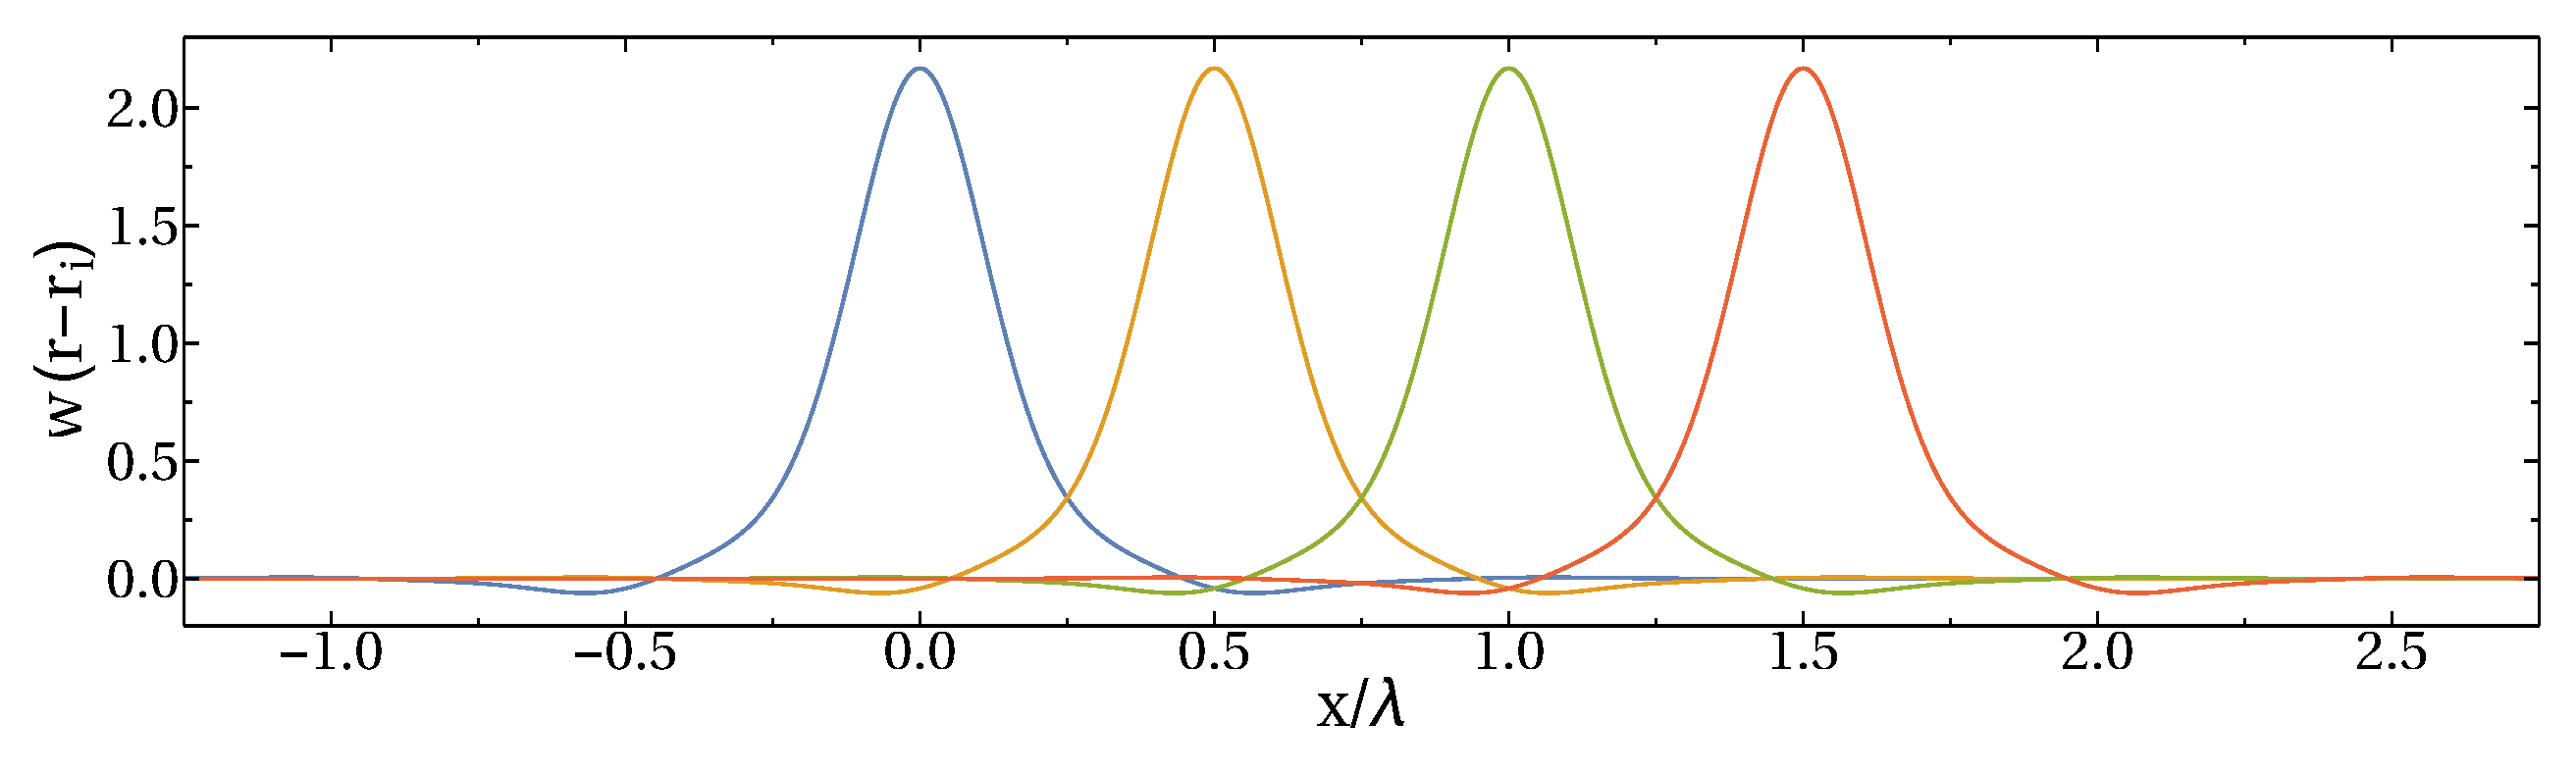
\includegraphics[width=1.0\textwidth]{Wannier1}
  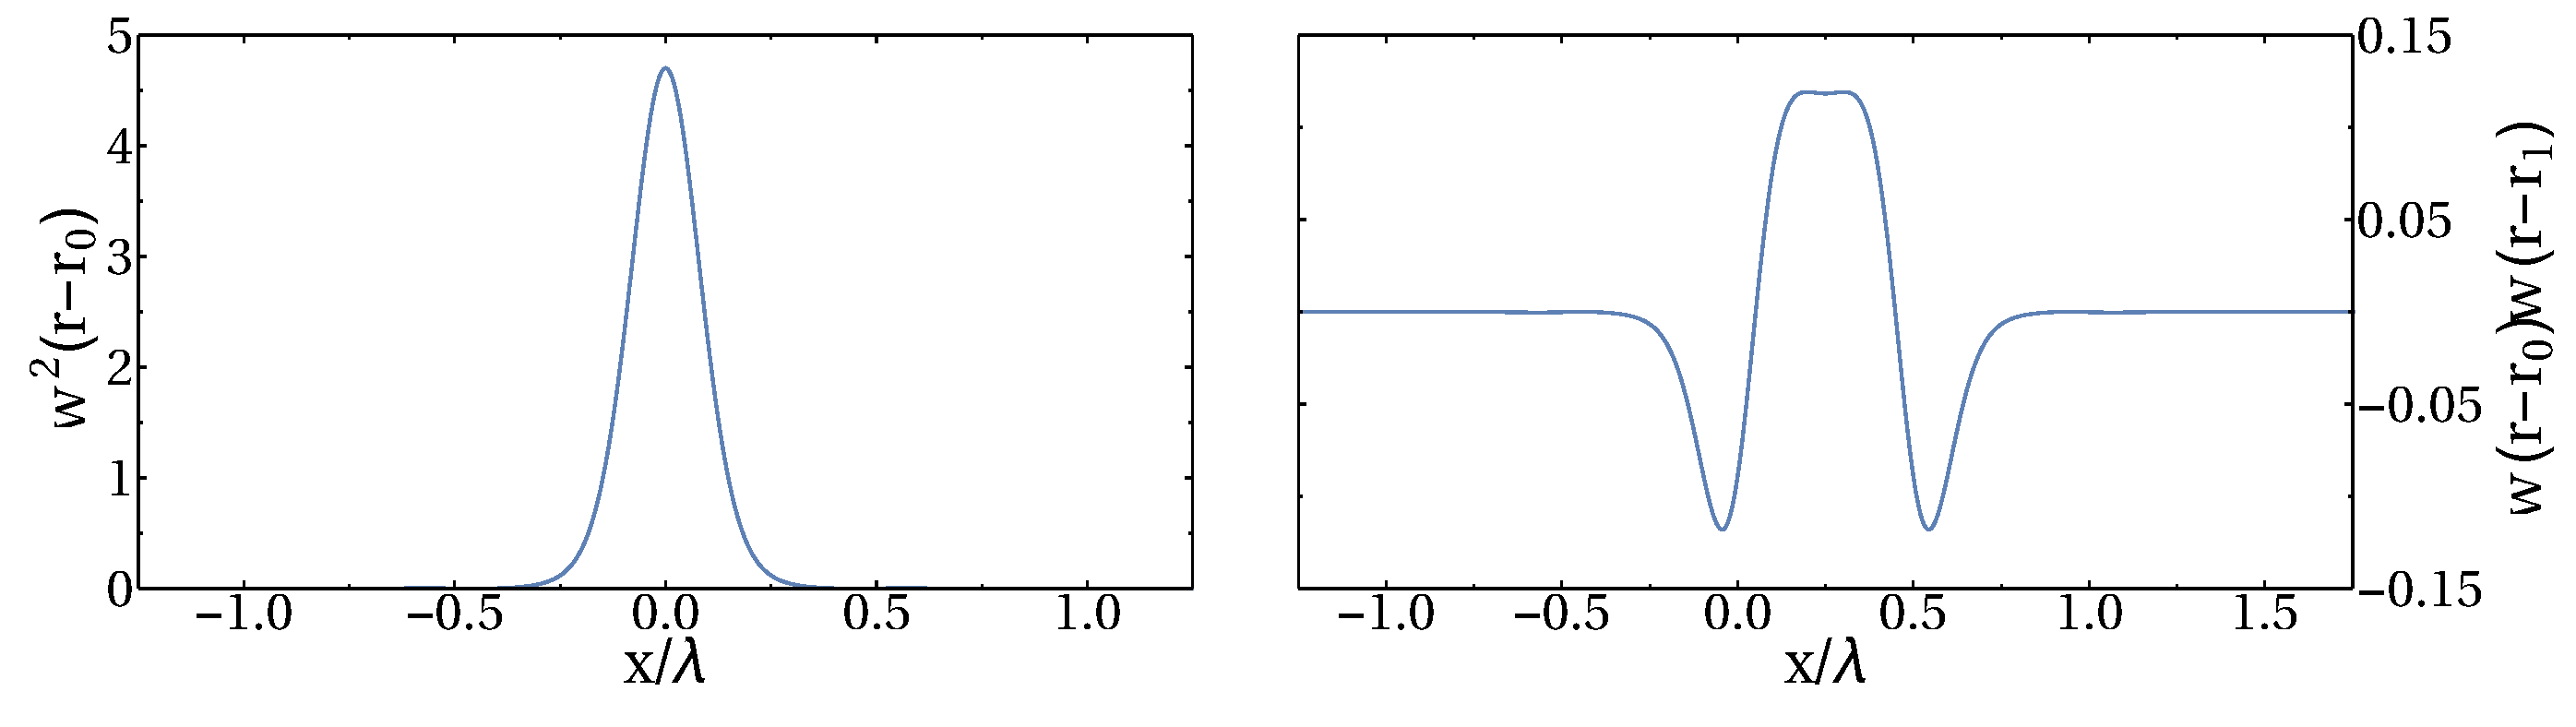
\includegraphics[width=1.0\textwidth]{Wannier2}
  \caption[Wannier Function Overlaps]{(a) The Wannier functions
    corresponding to four neighbouring sites in a 1D
    lattice. $\lambda$ is the wavelength of the trapping beams, thus
    lattice sites occur every $\lambda/2$. (Bottom Left) The square of
    a single Wannier function - this quantity is used when evaluating
    $\hat{D}$. It's much larger than the overlap between two
    neighbouring Wannier functions, but it is localised to the
    position of the lattice site it belongs to. (Bottom Right) The
    overlap of two neighbouring Wannier functions - this quantity is
    used when evaluating $\hat{B}$. It is much smaller than the square
    of a Wannier function, but since it's localised in between the
    sites, thus $\hat{B}$ can be maximised while $\hat{D}$ minimised
    by focusing the light in between the sites.}
  \label{fig:WannierOverlaps}
\end{figure}

\mynote{show the expansion into an FT}
In order to calculate the $J_{i,j}$ coefficients we perform numerical
calculations using realistic Wannier functions. However, it is
possible to gain some analytic insight into the behaviour of these
values by looking at the Fourier transforms of the Wannier function
overlaps, $\mathcal{F}[W_{0,1}](k)$, shown in Fig.
\ref{fig:WannierFT}b. This is because the light mode product,
$u_1^*(x) u_0(x)$, can be in general decomposed into a sum of
oscillating exponentials of the form $e^{i k x}$ making the integral
in Eq. \eqref{eq:Jcoeff} a sum of Fourier transforms of
$W_{0,1}(x)$. We consider both the detected and probe beam to be
standing waves which gives the following expressions for the $\hat{D}$
and $\hat{B}$ operators
\begin{eqnarray}
  \label{eq:FTs}
  \hat{D} =
  \frac{1}{2}[\mathcal{F}[W_0](k_-)\sum_m\hat{n}_m\cos(k_- x_m
    +\varphi_-)
    \nonumber\\ +\mathcal{F}[W_0](k_+)\sum_m\hat{n}_m\cos(k_+
    x_m +\varphi_+)], \nonumber\\ \hat{B} =
  \frac{1}{2}[\mathcal{F}[W_1](k_-)\sum_m\hat{B}_m\cos(k_- x_m
    +\frac{k_-d}{2}+\varphi_-)
    \nonumber\\ +\mathcal{F}[W_1](k_+)\sum_m\hat{B}_m\cos(k_+
    x_m +\frac{k_+d}{2}+\varphi_+)],
\end{eqnarray}
where $k_\pm = k_{0x} \pm k_{1x}$, $k_{(0,1)x} = k_{0,1}
\sin(\theta_{0,1}$), $\hat{B}_m=b^\dag_mb_{m+1}+b_mb^\dag_{m+1}$, and
$\varphi_\pm=\varphi_0 \pm \varphi_1$. The key result is that the
$\hat{B}$ operator is phase shifted by $k_\pm d/2$ with respect to the
$\hat{D}$ operator since it depends on the amplitude of light in
between the lattice sites and not at the positions of the atoms,
allowing to decouple them at specific angles.

\begin{figure}[htbp!]
  \begin{center}
    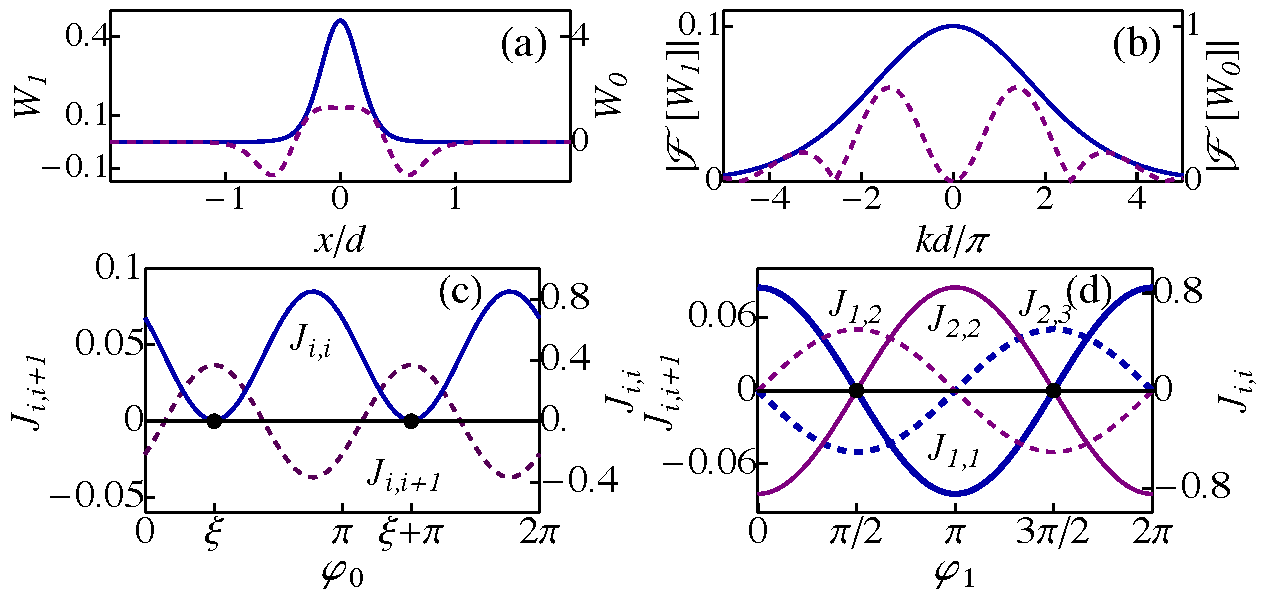
\includegraphics[width=\linewidth]{WF_S}
  \end{center}
  \caption[Wannier Function Fourier Transforms]{The Wannier function
    products: (a) $W_0(x)$ (solid line, right axis), $W_1(x)$ (dashed
    line, left axis) and their (b) Fourier transforms
    $\mathcal{F}[W_{0,1}]$. The Density $J_{i,i}$ and
    matter-interference $J_{i,i+1}$ coefficients in diffraction
    maximum (c) and minimum (d) as are shown as functions of standing
    wave shifts $\varphi$ or, if one were to measure the quadrature
    variance $(\Delta X^F_\beta)^2$, the local oscillator phase
    $\beta$. The black points indicate the positions, where light
    measures matter interference $\hat{B} \ne 0$, and the density-term
    is suppressed, $\hat{D} = 0$. The trapping potential depth is
    approximately 5 recoil energies.}
  \label{fig:WannierFT}
\end{figure}

The simplest case is to find a diffraction maximum where $J_{i,i+1} =
J_B$. This can be achieved by crossing the light modes such that
$\theta_0 = -\theta_1$ and $k_{0x} = k_{1x} = \pi/d$ and choosing the
light mode phases such that $\varphi_+ = 0$. Fig. \ref{fig:WannierFT}c
shows the value of the $J_{i,j}$ coefficients under these
circumstances. In order to make the $\hat{B}$ contribution to light
scattering dominant we need to set $\hat{D} = 0$ which from
Eq. \eqref{eq:FTs} we see is possible if $\varphi_0 = -\varphi_1 =
\arccos[-\mathcal{F}[W_0](2\pi/d)/\mathcal{F}[W_0](0)]/2$. This
arrangement of light modes maximizes the interference signal,
$\hat{B}$, by suppressing the density signal, $\hat{D}$, via
interference compensating for the spreading of the Wannier
functions. 

Another possibility is to obtain an alternating pattern similar
corresponding to a classical diffraction minimum. We consider an
arrangement where the beams are arranged such that $k_{0x} = 0$ and
$k_{1x} = \pi/d$ which gives the following expressions for the density
and interference terms
\begin{eqnarray}
  \label{eq:DMin}
	\hat{D} = \mathcal{F}[W_0](\pi/d) \sum_m (-1)^m \hat{n}_m
        \cos(\varphi_0) \cos(\varphi_1) \nonumber \\ \hat{B} =
        -\mathcal{F}[W_1](\pi/d) \sum_m (-1)^m \hat{B}_m
        \cos(\varphi_0) \sin(\varphi_1).
\end{eqnarray}
The corresponding $J_{i,j}$ coefficients are shown in
Fig. \ref{fig:WannierFT}d for $\varphi_0=0$. It is clear that for
$\varphi_1 = \pm \pi/2$, $\hat{D} = 0$, which is intuitive as this
places the lattice sites at the nodes of the mode $u_1(x)$. This is a
diffraction minimum as the light amplitude is also zero, $\langle
\hat{B} \rangle = 0$, because contributions from alternating
inter-site regions interfere destructively. However, the intensity
$\langle \ad_1 \a \rangle = |C|^2 \langle \hat{B}^2 \rangle$ is
proportional to the variance of $\hat{B}$ and is non-zero. 

\mynote{explain quadrature}
Alternatively, one can use the arrangement for a diffraction minimum
described above, but use travelling instead of standing waves for the
probe and detected beams and measure the light quadrature variance. In
this case $\hat{X}^F_\beta = \hat{D} \cos(\beta) + \hat{B}
\sin(\beta)$ and by varying the local oscillator phase, one can choose
which conjugate operator to measure.

\mynote{fix labels}
\begin{figure}[hbtp!]
	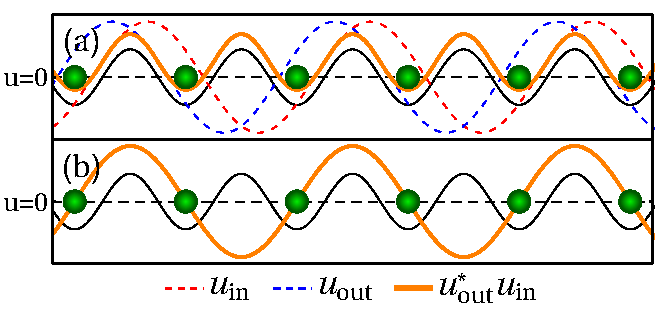
\includegraphics[width=\linewidth]{BDiagram}
	\caption[Maximising Light-Matter Coupling between Lattice
          Sites]{Light field arrangements which maximise coupling,
          $u_1^*u_0$, between lattice sites. The thin black line
          indicates the trapping potential (not to scale). (a)
          Arrangement for the uniform pattern $J_{m,m+1} = J_1$. (b)
          Arrangement for spatially varying pattern $J_{m,m+1}=(-1)^m
          J_2$; here $u_0=1$ so it is not shown and $u_1$ is real thus
          $u_1^*u_0=u_1$. \label{fig:BDiagram}}
\end{figure}

\subsection{Electric Field Stength}

The Electric field operator at position $\b{r}$ and at time $t$ is
usually written in terms of its positive and negative components:
\begin{equation}
  \b{\hat{E}}(\b{r},t) = \b{\hat{E}}^{(+)}(\b{r},t) + \b{\hat{E}}^{(-)}(\b{r},t),
\end{equation}
where
\begin{subequations}
  \begin{equation}
    \b{\hat{E}}^{(+)}(\b{r},t) = \sum_{\b{k}} \hat{\epsilon}_{\b{k}} 
    \mathcal{E}_{\b{k}} \a_{\b{k}} e^{-i \omega_{\b{k}} t + i \b{k} \cdot \b{r}},
  \end{equation}
  \begin{equation}
    \b{\hat{E}}^{(-)}(\b{r},t) = \sum_{\b{k}} \hat{\epsilon}_{\b{k}} 
    \mathcal{E}_{\b{k}} \a^\dagger_{\b{k}} e^{i \omega_{\b{k}} t - i \b{k} \cdot \b{r}},
  \end{equation}
\end{subequations}
$\hat{\epsilon}_{\b{k}}$ is a unit polarization vector, $\b{k}$ is the
wave vector,
$\mathcal{E}_{\b{k}} = \sqrt{\hbar \omega_{\b{k}} / 2 \epsilon_0 V}$,
$\epsilon_0$ is the free space permittivity, $V$ is the quantization
volume and $\a_\b{k}$ and $\a_\b{k}^\dagger$ are the annihilation and
creation operators respectively of a photon in mode $\b{k}$, and
$\omega_\b{k}$ is the angular frequency of mode $\b{k}$.

In Ref. \cite{Scully} it was shown that the operator
$\b{\hat{E}}^{(+)}(\b{r},t)$ due to light scattering from a single
atom located at $\b{r}^\prime$ at the observation point $\b{r}$ is
given by
\begin{equation}
  \label{eq:Ep}
  \b{\hat{E}}^{(+)}(\b{r},\b{r}^\prime,t) = \frac{\omega_a^2 d \sin \eta}{4 \pi
    \epsilon_0 c^2 |\b{r} - \b{r}^\prime|} \hat{\epsilon} \sigma^-
  \left( \b{r}^\prime, t - \frac{|\b{r} - \b{r}^\prime|}{c} \right),
\end{equation}
with a similar expression for
$\b{E}^{(-)}(\b{r},\b{r}^\prime,t)$. Eq. \eqref{eq:Ep} is valid only
in the far field, $\eta$ is the angle the dipole makes with
$\b{r} - \b{r}^\prime$, $\hat{\epsilon}$ is the polarization vector
which is perpendicular to $\b{r} - \b{r}^\prime$ and lies in the plane
defined by $\b{r} - \b{r}^\prime$ and the dipole, $\omega_a$ is the
atomic transition frequency, and $d$ is the dipole matrix element
between the two levels, and $c$ is the speed of light in vacuum.


We have already derived an expression for the atomic lowering
operator, $\sigma^-$, in Eq. \eqref{eq:sigmam} and it is given by
\begin{equation}
  \sigma^-(\b{r}, t) = - \frac{i} {\Delta_a} \sum_\b{k} g_\b{k}
  a_\b{k}(t) u_\b{k}(\b{r}).
\end{equation}
We will want to substitute this expression into Eq. \eqref{eq:Ep}, but
first we note that in the setup we consider the coherent probe will be
much stronger than the scattered modes. This in turn implies that the
expression for $\sigma^-$ will be dominated by this external
probe. Therefore, we drop the sum and consider only a single wave
vector, $\b{k}_0$, of the dominant contribution from the external
beam corresponding to the mode $\a_0$.

We now use the definititon of the atom-light coupling constant
\cite{Scully} to make the substitution
$g_0 a_0 = -i \Omega_0 e^{-i \omega_0 t} / 2$, where
$\Omega_0$ is the Rabi frequency for the probe-atom system. We now
evaluate the polarisation operator at the retarded time
\begin{equation}
  \sigma^- \left(\b{r}^\prime, t - \frac{|\b{r} - \b{r}^\prime|}{c} \right) =
  -\frac{\Omega_0}{2 \Delta_a} u_0 (\b{r}^\prime) \exp \left[-i \omega_0
    \left( t - \frac{|\b{r} - \b{r}^\prime|}{c} \right)\right].
\end{equation}
We are considering observation in the far field regime so
$|\b{r} - \b{r}^\prime| \approx r - \hat{\b{r}} \cdot
\b{r}^\prime$. We also consider the incoming, $\b{k}_0$, and the
outgoing, $\mathbf{k}_1$, waves to be of the same wavelength,
$|\b{k}_0| = |\b{k}_1| = k = \omega_0 / c$, hence
$(\omega_0 / c) |\b{r} - \b{r}^\prime| \approx k (r - \hat{\b{r}}
\cdot \b{r}^\prime) = \b{k}_1 \cdot (\b{r} - \b{r}^\prime )$ and
\begin{equation}
  \sigma^- \left(\b{r}^\prime, t - \frac{|\b{r} - \b{r}^\prime|}{c} \right) \approx
  -\frac{\Omega_0}{2 \Delta_a} u_0 (\b{r}^\prime) \exp \left[i
    \b{k}_1 \cdot (\b{r} - \b{r}^\prime ) - i \omega_0 t \right].
\end{equation}

The many-body version of the electric field operator is given by
\begin{equation}
  \b{\hat{E}}^{(+)}_N(\b{r},t) = \int \mathrm{d}^3 \b{r}^\prime
  \Psi^\dagger (\b{r}^\prime) \b{\hat{E}}^{(+)}(\b{r},\b{r}^\prime,t) \Psi(\b{r}^\prime),
\end{equation}
where $\Psi(\b{r})$ is the atomic matter-field operator. As before, we
expand this field operator using localized Wannier functions
corresponding to the lattice potential and keeping only the lowest
vibrational state at each site:
$\Psi(\b{r}) = \sum_i b_i w(\b{r} - \b{r}_i)$, where $b_i$ is the
annihilation operator of an atom at site $i$ with the coordinate
$\b{r}_i$. Thus, the relevant many-body operator is
\begin{subequations}
  \begin{equation}
    \b{\hat{E}}^{(+)}_N(\b{r},t) = \hat{\epsilon} C_E
    \sum_{i,j}^K \bd_i b_j \int \mathrm{d}^3 \b{r}^\prime
    w^* (\b{r}^\prime - \b{r}_i)  \frac{u_0
      (\b{r}^\prime)}{|\b{r} - \b{r}^\prime|} e^ {i \b{k}_1
      \cdot (\b{r} - \b{r}^\prime ) - i \omega_0 t }
    w(\b{r}^\prime - \b{r}_j),
  \end{equation}
  \begin{equation}
    C_E = -\frac{\omega_a^2 \Omega_0 d \sin \eta}{8 \pi \epsilon_0 c^2
      \Delta_a}
  \end{equation}
\end{subequations}
where $K$ is the number of illuminated sites. We now assume that the
lattice is deep and that the light scattering occurs on time scales
much shorter than atom tunneling. Therefore, we ignore all terms for
which $i \ne j$ and the remaining integrals become $\int \mathrm{d}^3
\b{r}_0 w^*(\b{r}_0 - \b{r}_i) f (\b{r})
w(\b{r}_0 - \b{r}_i) = f(\b{r}_i)$. The final form of
the many body operator is then
\begin{equation}
  \b{E}^{(+)}_N(\b{r},t) = \hat{\epsilon} C_E
  \sum_{j = 1}^K \hat{n}_j \frac{u_0 (\b{r}_j)}{|\b{r} -
    \b{r}_j|} e^ {i \b{k}_1 \cdot (\b{r} - \b{r}_j
    ) - i \omega_0 t },
\end{equation}
where $\hat{n}_i = b^\dagger_ib_i$ is the atom number operator at site
$i$. We will now consider the incoming probe to be a plane wave,
$u_0(\b{r}) = e^{i \b{k}_0 \cdot \b{r}}$, and we
approximate $|\b{r} - \b{r}_j| \approx r$ in the
denominator. Thus,
\begin{equation}
  \b{E}^{(+)}_N(\b{r},t) = \hat{\epsilon} C_E \frac{e^ {ikr - i\omega_0t}}{r}
  \sum_{j = 1}^K \hat{n}_j e^ {i (\b{k}_0 - \b{k}_1) \cdot \b{r}_j}.
\end{equation}
We note that this is exactly the same form of the optical field as
derived from a generalised Bose-Hubbard model which considers a fully
quantum light-matter interaction Hamiltonian \cite{mekhov2007prl,
  mekhov2007pra, mekhov2012}. We can even express the result in terms of
the $\hat{D} = \sum_j^K u_1^*(\b{r}_j) u_0(\b{r}_j)
\hat{n}_j$ formalism used in those works
\begin{equation}
  \b{E}^{(+)}_N(\b{r},t) = \hat{\epsilon} C_E \frac{e^
    {ikr - i\omega_0t}}{r} \hat{D}.
\end{equation}

The average light intensity at point $\b{r}$ at time $t$ is given
by the formula $I = c \epsilon_0 |E|^2/2$ and yields
\begin{equation}
  \langle I (\b{r}, t) \rangle = c \epsilon_0 \langle
  E^{(-)} (\b{r}, t) E^{(+)} (\b{r}, t) \rangle =
  \frac{c \epsilon_0}{r^2} C_E^2 \langle \hat{D}^* \hat{D} \rangle.
\end{equation}
The scattering is dominated by a uniform background for which $\langle
\hat{D}^* \hat{D} \rangle \approx N_K$ for a superfluid
\cite{mekhov2012}, where $N_K$ is the mean number of atoms in the
illuminated volume. Thus, the approximate number of photons scattered
per second can be obtained by integrating over a sphere
\begin{equation}
  n_{\Phi} = \frac{4 \pi c \epsilon_0}{3 \hbar \omega_a} \left(\frac{\omega_a^2
      \Omega_0 d}{8 \pi \epsilon_0 c^2 \Delta_a}\right)^2 N_K.
\end{equation}
In the Weisskopf-Wigner approximation it can be shown \cite{Scully}
that for a two level system the decay constant, $\Gamma$, is
\begin{equation}
  \Gamma = \frac{\omega_a^3 d^2}{3 \pi \epsilon_0 \hbar c^3}.
\end{equation}
Therefore, we can now express the quantity $n_{\Phi}$ as
\begin{equation}
  n_{\Phi} = \frac{1}{8} \left(\frac{\Omega_0}{\Delta_a}\right)^2 \frac{\Gamma}{2} N_K.
\end{equation}
Estimates of the scattering rate using real experimental parameters
are given in Table \ref{tab:photons}.

\begin{table}[!htbp]
  \centering
  \begin{tabular}{|c|c|c|}
    \hline
    Value & Miyake \emph{et al.} & Weitenberg \emph{et al.} \\ \hline
    $\omega_a$ & \multicolumn{2}{|c|}{$2 \pi \cdot 384$ THz}\\ \hline
    $\Gamma$ & \multicolumn{2}{|c|}{$2 \pi \cdot 6.07$ MHz} \\ \hline
    $\Delta_a$ & $2\pi \cdot 30$ MHz & $2 \pi \cdot 85$ MHz \\ \hline
    $I$ & $4250$ Wm$^{-2}$ & N/A \\ \hline
    $\Omega_0$ & 293$\times 10^6$ s$^{-1}$ & 42.5$\times 10^6$ s$^{-1}$ \\ \hline
    $N_K$ & 10$^5$ & 147 \\ \hline \hline
    $n_{\Phi}$ & $6 \times 10^{11}$ s$^{-1}$ & $2 \times 10^6$ s$^{-1}$ \\ \hline
  \end{tabular}
  \caption[Photon Scattering Rates]{ Rubidium data taken from
    Ref. \cite{steck}; Miyake \emph{et al.}: based on
    Ref. \cite{miyake2011}. The $5^2S_{1/2}$, $F=2 \rightarrow
    5^2P_{3/2}$, $F^\prime = 3$ transition of $^{87}$Rb is
    considered. For this transition the Rabi frequency is actually
    larger than the detuning and and effects of saturation should be
    taken into account in a more complete analysis. However, it is
    included for discussion. The detuning is said to be a few natural
    linewidths. Note that it is much smaller than $\Omega_0$. The Rabi
    fequency is $\Omega_0 = (d_\mathrm{eff}/\hbar)\sqrt{2 I / c
      \epsilon_0}$ which is obtained from definition of Rabi
    frequency, $\Omega = \mathbf{d} \cdot \mathbf{E} / \hbar$,
    assuming the electric field is parallel to the dipole, and the
    relation $I = c \epsilon_0 |E|^2 /2$. We used $d_\mathrm{eff} =
    1.73 \times 10^{-29}$ Cm \cite{steck}; Weitenberg \emph{et al.}:
    based on Ref. \cite{weitenberg2011, weitenbergThesis}. The
    $5^2S_{1/2} \rightarrow 5^2P_{3/2}$ transition of $^{87}$Rb is
    used. Ref. \cite{weitenberg2011} gives the free space detuning to
    be $\Delta_\mathrm{free} = - 2 \pi \cdot 45$
    MHz. Ref. \cite{weitenbergThesis} clarifies that the relevant
    detuning is $\Delta = \Delta_\mathrm{free} + \Delta_\mathrm{lat}$,
    where $\Delta_\mathrm{lat} = - 2 \pi \cdot 40$
    MHz. Ref. \cite{weitenbergThesis} uses a saturation parameter
    $s_\mathrm{tot}$ to quantify the intensity of the beams which is
    related to the Rabi frequency, $s_\mathrm{tot} = 2 \Omega^2 /
    \Gamma^2$ \cite{steck,foot}. We can extract $s_\mathrm{tot}$ for
    the experiment from the total scattering rate by
    $\Gamma_\mathrm{sc} = (\Gamma/2) (s_\mathrm{tot}) /
    (1+s_\mathrm{tot}+(2 \Delta / \Gamma)^2)$. A scattering rate of 60
    kHz per atom \cite{weitenberg2011} gives $s_\mathrm{tot} = 2.5$.}
  \label{tab:photons}
\end{table}
